\documentclass[a4paper,11pt]{exam}

\printanswers
\pagestyle{headandfoot}
\runningheadrule
%\firstpageheader{Math 115}{First Exam}{July 4, 1776}
\runningheader{}{Electronique numérique, Page \thepage\ / \numpages}{}
\firstpagefooter{}{}{}\runningfooter{}{ENSTA Bretagne}{JC Le Lann}

\usepackage{color} % defines a new color
\definecolor{SolutionColor}{rgb}{0.8,0.9,1} % light blue
\shadedsolutions % defines the style of the solution environment
% \framedsolutions % defines the style of the solution environment
% Defines the title of the solution environment:
\renewcommand{\solutiontitle}{\noindent\textbf{Solution:}\par\noindent}


\usepackage[utf8]{inputenc}
\usepackage[french]{babel}
\usepackage{amsmath}
\usepackage{graphicx}
\usepackage{float}
\restylefloat{table}

\title{BE : conception d'un accélérateur matériel\\pour le calcul de polynômes\\\textbf{solutions}}
\author{Electronique numérique 1A}

\begin{document}
\maketitle

On se propose ici de concevoir un accélérateur matériel, dédié au calcul de polynômes de rang 3. L'étude commence par une réflexion algorithmique, qui suggère des optimisations. Nous poursuivons la démarche par la manipulation abstraite de cet algorithme, à l'aide de \textit{graphes}. L'accélérateur concu par le suite se présente comme une microarchitecture, composée classiquement d'un automate de contrôle et d'un chemin de données.  On se limitera à des valeurs de x entières, codées sur 32 bits.

\section{Réflexion algorithmique}

La conception d'un accélérateur matériel naît souvent de la création d'un algorithme aux performances théoriques intéressantes (ex: compression par Transformée en Cosinus Discret), ou par
la découverte d'une reformulation intéressante (ex : multiplication de Karatsuba \footnote{Nous vous invitons à vous renseigner sur ces deux curiosités mathématiques}). Nous allons ici, en miniature, suivre cette démarche.\\
On considère un polynôme d'ordre 3 :
\begin{equation}
P_3(x)=a_3x^3+a_2x^2+a_1x+a_0
\end{equation}

\begin{questions}
  \question \textbf{Question} : Combien de multiplications et d'additions sont-elles nécessaires ?
    \begin{solution}
    Il en faut : 3+2+1 = 6 multiplications, et 3 additions.
    \end{solution}
  \question \textbf{Question} : A l'aide du schéma de Hörner, normalement connu, montrer que l'on peut réduire le nombre de ces opérations.
    \begin{solution}
    On peut réécrire le polynôme précédent de la manière suivante :
    \begin{align}
      P_3(x) &= x(a_3x^2+a_2x+a_1)+a_0 \\
             &=x(x(a_3x+a_2)+a_1)+a_0
    \end{align}
    On en déduit que sous cette forme, seulement 3 multiplications sont nécessaires (en plus des 3 additions).
    \end{solution}
\end{questions}

\section{Flot de données}
L'étude du flot de données (ou DFG : dataflow graph) permet d'établir les dépendances du calcul. On représente généralement ces dépendances à l'aide d'un graphe orienté : chaque noeud représente une opération (ici arithmétique) ou une entrée ou une sortie. Chaque arc entre deux noeuds est étiqueté par le nom de la variable qui circule du noeud source au noeud destination. Dans notre cas, le graphe est acyclique. Il indique clairement l'enchaînement des opérations, mais il s'agit encore d'une vision abstraite du calcul, indépendante de choix d'architecture matérielle. On peut toutefois noter que ce DFG peut être vu comme une première tentative de réalisation purement combinatoire du circuit (mais son chemin critique est très certainement rédhibitoire).

\begin{questions}
  \question \textbf{Question} : établir le graphe de flot de données issu du schéma de Hörner.
  \begin{solution}
      \begin{center}
        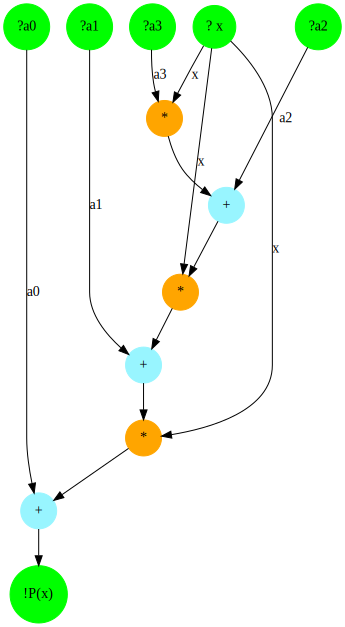
\includegraphics[scale=0.5]{dfg_horner.png}
      \end{center}
  \end{solution}
\end{questions}

\section{Ordonnancement. Assignation et partage des ressources}

La notion d'\textbf{ordonnancement} permet de découper le DFG en différentes étapes de calculs, appelées \textbf{control-step} (CSTEP). Prosaïquement, cela revient à dessiner différentes lignes qui représentent effectivement cette découpe du DFG.\\

Chacune des étapes s'exécute en un seul cycle d'horloge. Selon la durée physique du cycle d'horloge, il est toutefois possible de réaliser des découpes du DFG plus ou moins "longues" : plus le cycle est long, plus il est possible d'envisager de \textbf{chaîner} un ensemble d'opérations. A la fin du cycle, on devra veiller à échantillonner les données produites : formulé autrement, on peut dire que la découpe en CSTEPs détermine où devront se trouver les \textit{registres intermédiaires} de calcul.\\

En général, les opérateurs de calculs et les registres de calcul représentent la majeure partie de la surface occupée sur Silicium. Il est souvent souhaitable de les utiliser avec parcimonie et notamment de les partager dès que cela est possible. On réalise l'\textbf{assignation} des opérations aux opérateurs afin d'établir où se réaliseront effectivement les calculs du DFG abstrait. Bien évidemment, à la fin d'un CSTEP tous les opérateurs utilisés sont à nouveau disponibles pour le CSTEP suivant, ce qui donne des opportunités de partage de ressources entre opérations ordonnancées sur deux CSTEPs différents. Ces informations d'assignation peuvent être également annotées sur le DFG : à côté de l'opération abstraite du DFG, on peut indiquer sur quel opérateur matériel elle s'exécutera.\\

Avant même la phase d'assignation, le concepteur se donne par ailleurs un objectif en terme de nombre de ressources utilisées au total : c'est la phase d'\textbf{allocation de ressources}. Il peut se donner le droit d'utiliser tel nombre de multiplieurs, tel nombre d'additionneurs, tel nombre de registres, etc. Parmi les contraintes, on retrouve d'autres paramètres variés et en particulier la fréquence attendue du circuit. On se fixe ici une fréquence d'horloge de 100 Mhz.

\begin{questions}
  \question \textbf{Question 4} : on s'alloue 1 multiplieur et un additionneur. Le multiplieur a un temps de calcul de 7 ns et l'additionneur de 2 ns. Concernant les registres, on considère que leur temps de setup et old sont très inférieurs, et non significatifs par rapport aux opérateurs.  Proposer un ordonnancement qui vous semble judicieux. A combien de CSTEPS aboutissons-nous ?

  \begin{solution}
    On voit sur le DFG que le calcul de multiplication et d'addition se suivent. Le chemin critique de cet enchaînement est de $7+2=9 ns$. Or, la fréquence de fonctionnement des registres est de 100 Mhz soit un temps de cycle de 10 ns : ce bugdet de 10 ns laisse parfaitement le temps aux signaux de traverser à la fois le multiplieur et l'additionneur, dans un même cycle d'horloge. Cela est d'autant plus vrai que les temps de setup et hold sont considérés comme négligeables dans l'énoncé. On peut donc chaîner les opérateurs matériel dans le même cycle. Par contre, à la fin de cette portion (répétée) de circuit, il faudra échantillonner les signaux, dans des bascules D (registres). Le schéma suivant donne 3 CSTEPS. On suppose que les entrées et sorties sont également "clockées" (échantillonnées), ce qui est une bonne pratique.
    \begin{center}
      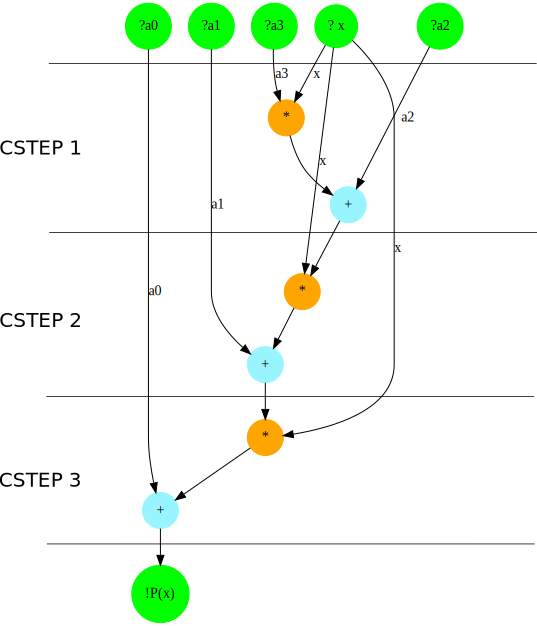
\includegraphics[scale=0.5]{dfg_horner_sched.png}
    \end{center}
  \end{solution}


  \question \textbf{Question 5} : réaliser l'assignation des ressources et notamment des registres.
  \begin{solution}
    On annote les ressources sur le schéma : il s'agit désormais d'opérateurs matériels et non plus d'opérations abstraites. Ces opérateurs peuvent être réutilisés à chaque cycle (CSTEP).
    De même un registre dont on n'a plus besoin peut être réutilisé. C'est le cas du regsitre R3, qui contient initialement le premier coefficient lu. Après cette lecture, on peut utiliser R3 pour les calculs des variables temporaires (intermédiaires) de calcul.
    \begin{center}
      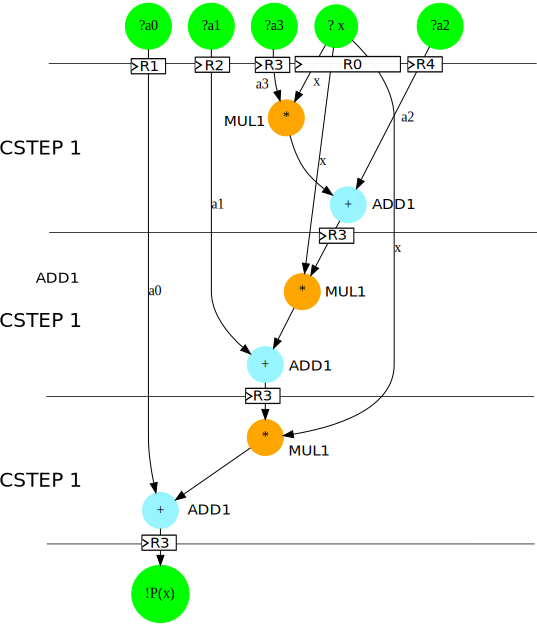
\includegraphics[scale=0.4]{dfg_horner_binding.png}
    \end{center}
  \end{solution}
\end{questions}

\section{Microarchitecture : automate de contrôle et datapath}
Dès lors qu'un ordonnancement est choisi, il est alors aisé de décrire un automate et un chemin de donnée. L'automate permet de séquencer les différentes étapes. Il réalise en outre, pour chacune d'entre elles, les actions appropriées. A l'issue de l'assignation, ces actions reviennent à contrôler les multiplexeurs d'un chemin de données (datapath) : ces multiplexeurs servent soit à échantillonner une donnée à l'entrée d'un registre, soit à router une donnée vers un opérateur matériel.\\

\begin{questions}
  \question \textbf{Question 6} : dessiner l'automate de contrôle.
  \begin{solution}
    \begin{center}
      \includegraphics[scale=0.4]{fsm.png}
    \end{center}
  \end{solution}
  \question \textbf{Question 7} : dessiner un chemin de données
    \begin{solution}
      Pour déterminer le chemin de données (datapath), on observe le DFG ordonnancé et alloué (question 5). Il s'agit essentiellement de déterminer les opérandes des opérateurs. Prenons le Multiplieur MUL1 : on voit que ses opérandes sont R0 et R3 lors du CSTEP 1, et à nouveau R0 et R3 aux CSTEPs 2 et 3. Le chemin entre les registres et l'entrée de MUL1 est donc très simple et direct. Observons maintenant ADD1 :
      \begin{itemize}
        \item dans le CSTEP 1, ADD1 opère sur le résultat combinatoire de MUL1 et sur R4
        \item dans le CSTEP 2, ADD1 opère sur le résultat combinatoire de MUL1 et sur R2
        \item dans le CSTEP 3, ADD1 opère sur le résultat combinatoire de MUL1 et sur R1
      \end{itemize}
      On peut en déduire que pour assurer ces 3 fonctionnements, il est nécessaire d'adjoindre un multiplexeur sur le second opérande de ADD1, dont les sources sont R4,R2 et R1.
      Notons que nos deux opérateurs sont commutatifs, ce qui a grandement simplifié notre analyse. On en déduit une version, encore incomplète, du datapath, présentée la figure suivante.
      \begin{center}
        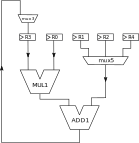
\includegraphics[scale=0.4]{datapath_primitif.png}
      \end{center}
      Quelques détails restent à régler : comment sont acheminés les entrées et calculs intermédiaires, vers ces registres ? Il faut bien penser à l'échantillonnage des entrées et leur stockage tout au long du calcul. Là encore on repose sur un multiplexeur, dont la commande peut jouer ce rôle. Afin de ne pas modifier la donnée stockée (potentiellement ré-échantillonnée à chaque cycle), on fait ainsi "recirculer" la donnée de la sortie Q à l'entrée D des bascules.
      Désormais notre datapath est complet. Reste à déterminer les instants de contrôles des multiplexeurs, émis par le contrôleur (fsm).
      \begin{center}
        \includegraphics[scale=0.4]{datapath.png}
      \end{center}

      On numérote les entrées des multiplexeurs : ces valeurs correspondront aux valeurs du signal de commande qu'il faudra envoyer au multiplexeur pour qu'il fasse passer l'entrée correspondante sur sa sortie. Cela nous permettra de piloter le cheminement des données (question suivante).
      \begin{center}
        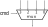
\includegraphics[scale=0.6]{mux.png}
      \end{center}
    \end{solution}

  \question \textbf{Question 8} : compléter l'automate pour indiquer les actions réalisées dans chaque état.
  \begin{solution}
    On se propose de présenter cet automate sous la forme tabulée suivante. Ce tableau fait apparaître les \textit{transfert de registres}, ainsi que les micro-actions correspondantes, sur les multiplexeurs.

    \begin{tabular}{|c | c | c | c|}
      \hline
      état & effet algorithmique & transferts de registres & commandes des multiplexeurs \\
      \hline
      ~   & arrivée des données & $R0 <= x$                 & $cmd_0 <= 1$                  \\
      ~   & ~                   & $R1 <= a_0$               & $cmd_1 <= 1$                  \\
      S0  & ~                   & $R2 <= a_1$               & $cmd_2 <= 1$                  \\
      ~   & ~                   & $R3 <= a_3$               & $cmd_3 <= 1$                  \\
      ~   & ~                   & $R4 <= a_2$               & $cmd_4 <= 1$                  \\
      ~   & ~                   & ~                         & $cmd_5 <= 1$                  \\
      \hline
      ~   & ~                   & ~                         & $cmd_0 <= 0$                  \\
      ~   & ~                   & ~                         & $cmd_1 <= 0$                  \\
      S1  & ~ $t_1=a_3*x+a_2$   & ~                         & $cmd_2 <= 0$                  \\
      ~   & ~                   & $R3 <= (R3*R0)+R4$        & $cmd_3 <= 2$                  \\
      ~   & ~                   & ~                         & $cmd_4 <= 0$                  \\
      ~   & ~                   & ~                         & $cmd_5 <= 0$                  \\
      \hline
      ~   & ~                   & ~                         & $cmd_0 <= 0$                  \\
      ~   & ~                   & ~                         & $cmd_1 <= 0$                  \\
      S2  & ~ $t_2=t_1*x+a_1$   & $R3 <= (R3*R0)+R2$        & $cmd_2 <= 0$                  \\
      ~   & ~                   & ~                         & $cmd_3 <= 2$                  \\
      ~   & ~                   & ~                         & $cmd_4 <= 0$                  \\
      ~   & ~                   & ~                         & $cmd_5 <= 1$                  \\
      \hline
      ~   & ~                   & ~                         & $cmd_0 <= 0$                  \\
      ~   & ~                   & ~                         & $cmd_1 <= 0$                  \\
      S3  & ~ $P(x)=t_2*x+a_0$  & $R3 <= (R3*R0)+R2$        & $cmd_2 <= 0$                  \\
      ~   & ~                   & ~                         & $cmd_3 <= 2$                  \\
      ~   & ~                   & ~                         & $cmd_4 <= 0$                  \\
      ~   & ~                   & ~                         & $cmd_5 <= 2$                  \\
      \hline
    \end{tabular}
    Quelques remarques :
    \begin{itemize}
      \item On notera au passage que ces transferts de registres ressemblent à s'y méprendre à un langage de programmation de bas niveau : l'assembleur. Toutefois, nos transferts de registres sont plus puissants que l'assembleur : plusieurs transferts peuvent avoir lieu en même temps, en parallèle ,alors qu'en assembleur traditionnel chaque tranfert se fait séquentiellement.
      \item L'opération de multiplication suivie d'une addition est si fréquente dans le domaine scientifique, qu'il existe un opérateur dédié : le MULACC. Il est présent notamment dans les processeurs de traitement du signal, appelés DSP (digital signal processors, les plus connus étant ceux de Texas Instruments). Les FPGA modernes, possèdent en plus de leur matrice de LUTs, un ensemble de tels opérateurs optimisés.
    \end{itemize}
  \end{solution}
\end{questions}

\section{Dimensionnement des registres}

Une difficulté récurrente lorsqu'on traduit un algorithme en Microarchitecture réside dans le dimensionnement des signaux, c'est-à-dire la détermination du nombre de bits nécessaires à la représentation des nombres, sans perte d'information préjudiciable. On parle aussi de leur \textit{dynamique}. Il y a perte d'information lors d'une troncature (élimination brutale de bits à un certain rang).

\begin{itemize}
  \item \textbf{Question 9} : soient deux signaux $s_n$ et $s_{n'}$ entiers codés respectivement sur $n$ et $n'$ bits. Déterminer le nombre de bits nécessaires à l'addition $s_n+s_{n'}$, sans perte d'information.
  \begin{solution}
    Par exemple, avec $n=8$ et $n'=8$, $s_n,s_{n'} \in \{0..255\}$ et $s_n+s_{n'} \in \{0..510\}$. On se convainc facilement que le nombre de bits pour le résultat de l'addition est $max(n,n')+1$.
  \end{solution}
  \item \textbf{Question 10} : même question pour $s_n*s_{n'}$.
  \begin{solution}
    Pour la multiplication le résultat est $n+n'$.
  \end{solution}
  \item \textbf{Question 11} : en déduire la dynamique des signaux apparaissant dans le datapath.
  \begin{solution}
A la fin de chaque CSTEP, la dynamique des signaux calculés augmente. Si chaque entrée est codée sur un même nombre $n$ de bits :
  \begin{itemize}
    \item CSTEP 1 : R3 nécessite $2n+1$ bits
    \item CSTEP 2 : R3 nécessite $(2n+1)+n+1=3n+2$ bits
    \item CSTEP 3 : R3 nécessite $(3n+2)+n+1=4n+3$ bits
  \end{itemize}
  A titre d'exemple, partant de $n=8$ bits, on obtient $35$ bits nécessaires en sortie.
  \end{solution}
\end{itemize}

\section{Codage VHDL}

Le code VHDL de cet accélérateur est fourni sur Moodle, ainsi qu'un banc de test.

\begin{itemize}
  \item \textbf{Question 12} : observez attentivement le code de l'accélérateur. Discutez avec votre encadrant afin de bien vérifier que vous avez compris la correspondance avec vos schémas précédents.
\end{itemize}

Le banc de test réalise tout d'abord la configuration de l'accélérateur, par l'envoi des paramètres du polynôme, puis réalise le calcul de $P_3(x)$ pour une succession de valeurs $x$.

\begin{itemize}
  \item \textbf{Question 13} : observez attentivement le code du banc de test. Discutez avec votre encadrant afin de bien vérifier que vous avez compris son fonctionnement.
\end{itemize}

\end{document}
